%%%%%%%%%%%%%%%%%%%%%%%%%%%%%%%%%%%%%%%%%
% University/School Laboratory Report
% LaTeX Template
% Version 3.1 (25/3/14)
%
% This template has been downloaded from:
% http://www.LaTeXTemplates.com
%
% Original author:
% Linux and Unix Users Group at Virginia Tech Wiki 
% (https://vtluug.org/wiki/Example_LaTeX_chem_lab_report)
%
% License:
% CC BY-NC-SA 3.0 (http://creativecommons.org/licenses/by-nc-sa/3.0/)
%
%%%%%%%%%%%%%%%%%%%%%%%%%%%%%%%%%%%%%%%%%

\documentclass{article}
\usepackage[utf8]{inputenc}
\usepackage{appendix}
\usepackage[T1]{fontenc}
\usepackage{siunitx} % Provides the \SI{}{} and \si{} command for typesetting SI units
\usepackage{graphicx} % Required for the inclusion of images
\usepackage{natbib} % Required to change bibliography style to APA
\usepackage{amsmath} % Required for some math elements 
\usepackage{caption}
\usepackage{tikz}

\usetikzlibrary{arrows,automata, positioning}

\usepackage{import}

\setlength\parindent{0pt} % Removes all indentation from paragraphs

\title{Prova Finale di Reti Logiche 2020/2021} % Title
\author{Vincenzo Greco} % Author name
\date{May 16th, 2021}

\begin{document}
\maketitle % Insert the title, author and date
\begin{center}
\begin{tabular}{l r}
Matricola: & 916368\\ % Partner names
Codice Persona: & 10683567\\
Docente: & Salice Fabio	 % Instructor/supervisor
\end{tabular}
\end{center}

\section{Requisiti del Progetto}

Il progetto richiesto consiste nell'implementazione in VHDL dell metodo di \textbf{
equalizzazione dell’istogramma di una immagine}.\\
Data un'immagine salvata in memoria viene chiesto al componente di:
\begin{enumerate}
\item Accedere ad una memoria RAM per recuperare il numero di righe e colonne di pixel di cui è composta l'immagine
\item Iterare nella memoria per trovare minimo e massimo dei valori dei pixel
\item Applicare l'equalizzazione ad ogni pixel dell'immagine
\item Salvare in memoria ogni pixel equalizzato a partire dalla posizione successiva rispetto all'ultimo pixel della matrice fornita
\end{enumerate}

La massima grandezza della matrice dell' immagine è \(128 * 128\).\\
Inoltre, l'implementazione deve essere in grado di gestire un segnale di Reset. L'implementazione deve essere sintetizzata con target FPGA xc7a200tfbg484-1.

\newpage
\noindent

%----------------------------------------------------------------------------------------
%	SECTION 2
%----------------------------------------------------------------------------------------

\section{Implementazione}

\subsection{Descrizione ad Alto Livello}

Da un'ottica di alto livello, l'implementazione esegue i seguenti passi:

\begin{enumerate}
\item Carica il numero di righe e colonne della matrice dei pixel dalla RAM
\item Esegue la ricerca di massimi e minimi:
\item Calcola il valore dello shift.
\item Per ogni pixel in memoria calcola il valore del pixel equalizzato e lo salva in RAM
\item Ad operazione conclusa il componente comunica il suo stato di done fin quando non verrà indicato che la prossima immagine è disponibile all' equalizzazione
\end{enumerate}

\subsection{Interpretazioni personali della specifica}

\begin{itemize}
    \item Nel caso fosse letto un valore maggiore di righe e/o colonne rispetto a quello consentito, questo verrà salvato ugualmente come il massimo consentito dalla specifica (128). Nel caso di presenza di valori in RAM oltre l' indice "righe x colonne + 2", questi verranno totalmente ignorati e, nel caso, sovrascritti.
    \item Per l'implementazione si è scelto di supporre il Reset asincrono rispetto al segnale di clock.
\end{itemize}

\subsection{Macchina a Stati Finiti}

La FSM è stata realizzata con specifica behavioural mediante due processi: \texttt{STATE} e \texttt{DELTA\_LAMBDA}: 
\begin{itemize}
    \item Il processo \texttt{STATE} è il processo che si occupa di cambiare lo stato sul fronte di salita del clock e di portare la macchina nello stato di reset se il segnale \texttt{I\_RST} fosse rilevato.
    \item Il processo \texttt{DELTA\_LAMBDA} è invece il processo combinatorio che calcola le uscite e lo stato validi per il prossimo fronte di salita del clock.
    \item L'implementazione dello shift è stata fatta tramite controllo di soglia in modo da poter risparmiare sulla complessità delle operazioni effettuate avendo anche un controllo maggiore sul risultato. 
\end{itemize}

Gli stati della FSM sono:

\begin{itemize}
\item \texttt{RST}: Stato in cui la macchina si prepara che il segnale \texttt{i\_start} venga portato alto per poter iniziare l'esecuzione. Questo stato si occupa anche di portare i segnali interni in uno stato consistente per l'esecuzione. In particolare il massimo e il minimo verranno inizializzati rispettivamente al valore minimo e massimo così da poter essere direttamente confrontati con il valore del primo pixel letto da RAM.
\item \texttt{SAVE\_COLUMN}: Stato in cui si legge dalla RAM l'indirizzo 0 della memoria che corrisponde al numero di colonne che compongono l'immagine. Il valore salvato sarà il minimo fra quello fronito da \texttt{i\_data} e 128. Nel caso il valore fosse 0 il processo si porterà nello stato di \texttt{DONE}.
\item \texttt{SAVE\_ROW}: Stato in cui si legge dalla RAM l'indirizzo 1 della memoria che corrisponde al numero di righe che compongono l'immagine. Il valore salvato sarà il minimo fra quello fronito da \texttt{i\_data} e 128. Nel caso il valore fosse 0 il processo si porterà nello stato di \texttt{DONE}.
\item \texttt{SAVE\_PIXEL}: Stato in cui si legge il valore del pixel puntato sulla RAM. Questo valore verrà confrontato con massimo e minimo attuali per, nel caso, aggiornarli.
\item \texttt{LOOP\_SAVE}: Stato in cui decide se siano stati letti tutti i valori della matrice di pixel dalla RAM.
\begin{itemize}
    \item Se non si è porata a termine la scansione di tutti pixel il processo tornerà nello stato \texttt{SAVE\_PIXEL}.
    \item Se tutti i pixel sono stati scansionati verrà calcolato il delta tramite l'operazione \(\texttt{DELTA} = max - min\).
\end{itemize}
\item \texttt{CALC\_SHIFT}: Stato in cui si calcola \(shift = 8-  {\lfloor}(LOG_2(\texttt{DELTA} +1)){\rfloor}\) tramite controllo di soglia.
\item \texttt{EQUALIZE\_PIXEL}: Stato in cui si calcola il valore del pixel equalizzato come \(valore\_pixel\_equalizzato = (valore\_pixel\_corrente - min) \ll shift\)
\item \texttt{SAVE\_PIXEL\_EQUALIZED}: Stato in cui viene salvato in memoria il valore \(nuovo\_valore = \min_{} (255, valore\_pixel\_equalizzato)\) partendo dall' indirizzo \(righe * colonne + 2\)
\item \texttt{LOOP\_SAVE\_EQUALIZED}: Stato in cui si decide se siano stati equalizzati tutti i pixel della matrice
\begin{itemize}
    \item Se non si è porata a termine l'equalizzazione di tutti i pixel il processo tornerà nello stato \texttt{EQUALIZE\_PIXEL}.
    \item Se tutti i pixel sono stati equalizzati verrà il processo si porterà nello stato di \texttt{DONE}.
\end{itemize}
\item \texttt{DONE}: Stato in il segnale \texttt{O\_DONE} verrà portato alto fin quando il segnale \texttt{i\_start} non venga portato basso per tornare poi allo stato di \texttt{RST}.
\end{itemize}

Nella figura a seguito è riportato il disegno dell'automa.


\begin{center}
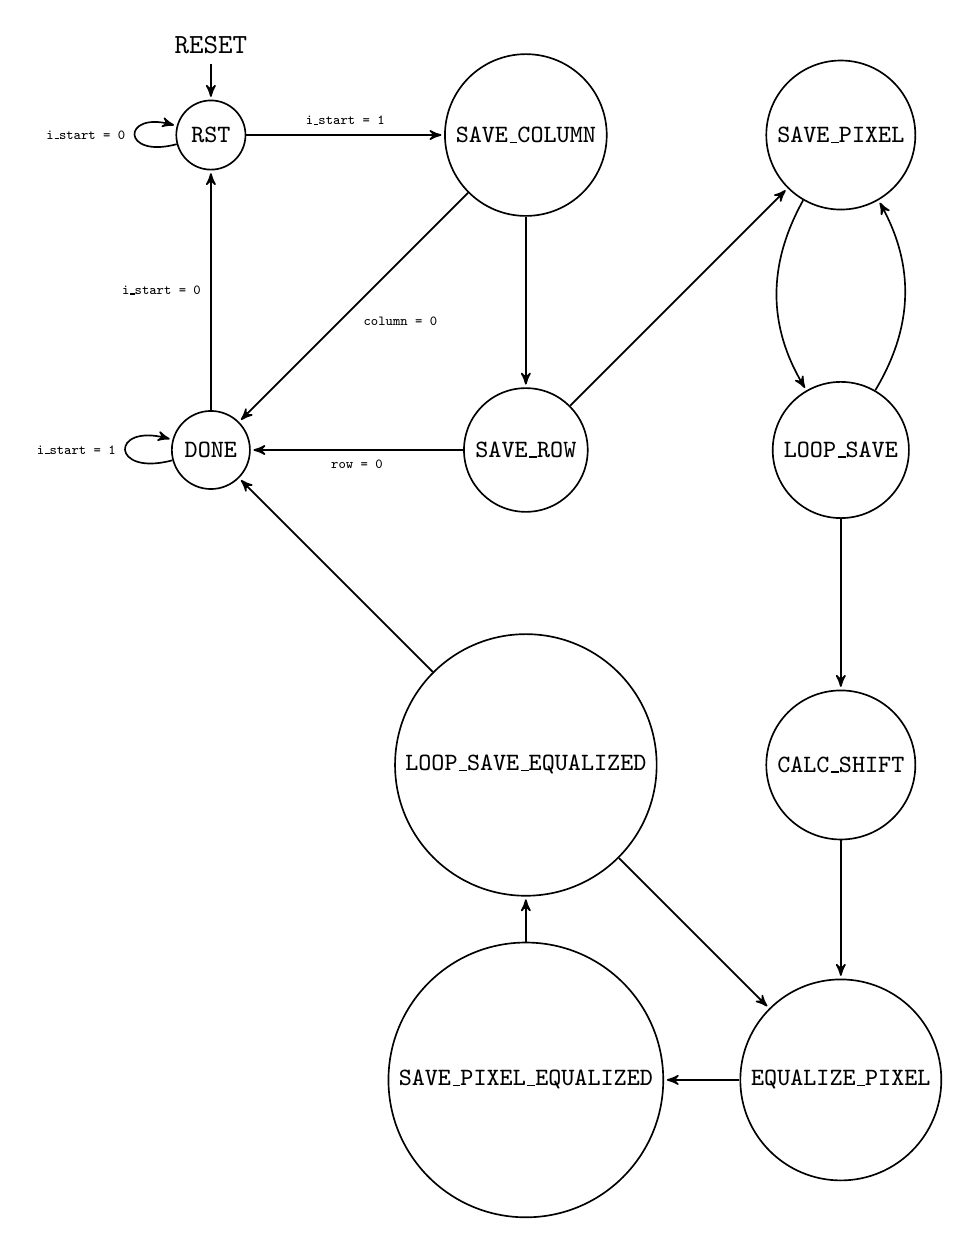
\begin{tikzpicture}[->,>=stealth',shorten >=1pt,auto,node distance=4cm,
                    semithick, initial where=above, initial text={\texttt{RESET}}]

  \tikzstyle{every state} = [font=\small]
  \node[initial,state] (A)                  {\texttt{RST}};
  \node[state]         (B) [right of=A] 	{\texttt{SAVE\_COLUMN}};
  \node[state]         (C) [below of=B] 	{\texttt{SAVE\_ROW}};
  \node[state]         (D) [right of=B] 	{\texttt{SAVE\_PIXEL}};
  \node[state]         (E) [below of=D]     {\texttt{LOOP\_SAVE}};
  \node[state]         (F) [below of=E]     {\texttt{CALC\_SHIFT}};
  \node[state]         (G) [below of=F]     {\texttt{EQUALIZE\_PIXEL}};
  \node[state]         (H) [left of=G]      {\texttt{SAVE\_PIXEL\_EQUALIZED}};
  \node[state]         (I) [left of=F]      {\texttt{LOOP\_SAVE\_EQUALIZED}};
  \node[state]         (J) [below of=A]     {\texttt{DONE}};

  \path (A) edge                    node {\tiny\texttt{i\_start = 1}} (B)
 	    (A) edge    [loop left]     node {\tiny\texttt{i\_start = 0}} (A)
        (B) edge                    node {} (C)
        (B) edge                    node {\tiny\texttt{column = 0}} (J)
        (C) edge                    node {} (D)
        (C) edge                    node {\tiny\texttt{row = 0}} (J)
        (D) edge    [bend right]	node {} (E)
        (E) edge 			        node {} (F)
        (E) edge 	[bend right]	node {} (D)
        (F) edge 		    	    node {} (G)
        (G) edge 			        node {} (H)
        (H) edge			        node {} (I)
        (I) edge			        node {} (J)
        (I) edge	        		node {} (G)
        (J) edge			        node {\tiny\texttt{i\_start = 0}} (A)
        (J) edge	[loop left]		node {\tiny\texttt{i\_start = 1}} (J);
\end{tikzpicture}
\end{center}

\newpage

\section{Test Benches}
\label{test}

I test sono stati effettutati allo scopo di trovari eventuali criticità del componente

\begin{itemize}
\item Segnale di \texttt{RESET} asincrono rispetto al clock
\item Valore di righe e/o colonne a 0 controllando che quindi nessun valore in RAM venga modificato
\item Matrice di pixel 1 x 1 e 128 x 128 per testare le dimensioni limite dell' immagine
\item Altri test bench vari generati casualmente, mantenendo comunque la validità della specifica
\item Testata la totale assenza di modifiche in memoria oltre quelle necessarie al implementazione della specifica richiesta
\end{itemize}

Per tutti i test svolti è stata effettuata la simulazione behavioural e successivamente la simulazione functional e timing post-synthesis, tutte con successo.

\section{Risultati Sperimentali}
\label{risultati}

\subsection{Report di Sintesi}

Dal punto di vista dell'area la sintesi riporta il seguente utilizzo dei componenti:
\begin{itemize}
\item LUT: 173 (0.13\% del totale)
\item FF: 112 (0.04\% del totale)
\end{itemize}

\subsection{Risultato dei Test Bench}

Lavorando sul testing si è anche provato a variare il periodo di clock, confermando che, non solo l'implementazione mantiene il suo funzionamento anche a \SI{1}{\ns} nella simulazione Behavioural e \SI{2}{\ns} nella simulazione Post-Synthesis, ma anche che la macchina non presenti risultati inattesi o inconsistenti. Test inferiori a \SI{1}{\ns} non sono stati effettuati.

\section{Conclusioni}

Avendo passato la totalità dei test sia scritti manualmente, che generati, che ricevuti attraverso beep o altri canali di comunicazione, posso affermare con una certa confidenza che l'implementazione rispetti tutte le specifiche indicate.
\end{document}
